\documentclass[twoside,a4paper]{book}
\usepackage{graphicx}
\usepackage{hyperref}
\usepackage{amsmath}
\usepackage{amssymb}
\usepackage{textcomp}
\usepackage[utf8]{inputenc}
\usepackage[polish]{babel}
\usepackage[T1]{fontenc}
\usepackage{standalone}
\usepackage{array}
% pakiet stosowany do url'i w bibliografii, zamienia odnośniki na ładnie sformatowane
\usepackage{url}
% pakiety służące do numerowania i tworzenia algorytmów
\usepackage{algorithmic}
\usepackage{algorithm}
% redefinicja etykiety nagłówkowej listy algorytmów, domyślna jest po angielsku
\renewcommand{\listalgorithmname}{Spis algorytmów}

\usepackage[section]{placeins}
\usepackage{pdfpages}

% pakiet do wyliczania skali, przydatny przy dużych obrazkach
\usepackage{pgf}
% pakiet służący do automatycznego sortowania odnośników do bibliografii
\usepackage[sort]{natbib}
% tworzenie listingów
\usepackage{listings}
% tworzenie figur wewnątrz figur
\usepackage{subfig}
% do automatycznego skracania nazw rozdziałów i podrozdziałów używanych w nagłówkach strony by mieściły się w jednej linii
\usepackage[fit]{truncate}
% fancyhdr - ładne nagłówki, definicja wyglądu nagłówka, numery stron będą umieszczane w nagłówku po odpowiedniej stronie
\usepackage{fancyhdr}
\pagestyle{fancy}
\renewcommand{\chaptermark}[1]{\markboth{#1}{}}
\renewcommand{\sectionmark}[1]{\markright{\thesection\ #1}}



\fancyhf{}
\fancyhead[LE,RO]{\bfseries\thepage}
% tutaj ograniczamy szerokość pola w nagłówku zawierającego nazwę rozdziału/podrozdziału do 95% szerokości strony
% redefinicja sposobu prezentacji nazw domyślnie wypisywanych wielkimi literami (np. domyślnie w nagłówku Spis treści będzie miał postać SPIS TREŚCI)
% Uwaga! to może popsuć wielkie litery w ogóle! Jak coś nie działa należy usunąć \nouppercase{} z poniższych definicji
\fancyhead[LO]{\nouppercase{\bfseries{\truncate{.95\headwidth}{\rightmark}}}}
\fancyhead[RE]{\nouppercase{\bfseries{\truncate{.95\headwidth}{\leftmark}}}}
\renewcommand{\headrulewidth}{0.5pt}
\renewcommand{\footrulewidth}{0pt}

% definicja typu prostego wymagana przez pierwsze strony rozdziałów itp.
% powyższe reguły niestety tych stron nie dotyczą, gdyż Latex automatycznie przełącza je pomiędzy fancy a plain
% w tym wypadku eliminujemy nagłówki i stopki na stronach początkowych
\fancypagestyle{plain}{%
 \fancyhead{}
 \fancyfoot{}
 \renewcommand{\headrulewidth}{0pt}
 \renewcommand{\footrulewidth}{0pt}
}

\parskip 0.05in


% makro umożliwiające otaczanie symboli okręgami
\usepackage{tikz}
% brak justowania tekstu (bazą okręgu będzie linia tekstu)
\newcommand*\mycirc[1]{%
  \begin{tikzpicture}
    \node[draw,circle,inner sep=1pt] {#1};
  \end{tikzpicture}}

% pionowe justowanie tekstu, środek okręgu pokrywa się ze środkiem tekstu
\newcommand*\mycircalign[1]{%
  \begin{tikzpicture}[baseline=(C.base)]
    \node[draw,circle,inner sep=1pt](C) {#1};
  \end{tikzpicture}}

% zmiana nazwy twierdzeń i lematów
\newtheorem{theorem}{Twierdzenie}[section]
\newtheorem{lemma}[theorem]{Lemat}

% tworzenie definicji dowodu
\newenvironment{proof}[1][Dowód]{\begin{trivlist}
\item[\hskip \labelsep {\bfseries #1}]}{\end{trivlist}}
% \newenvironment{definition}[1][Definicja]{\begin{trivlist}
% \item[\hskip \labelsep {\bfseries #1}]}{\end{trivlist}}
% \newenvironment{example}[1][Przykład]{\begin{trivlist}
% \item[\hskip \labelsep {\bfseries #1}]}{\end{trivlist}}
% \newenvironment{remark}[1][Uwaga]{\begin{trivlist}
% \item[\hskip \labelsep {\bfseries #1}]}{\end{trivlist}}

% definicja czarnego prostokąta zwyczajowo dodawanego na koniec dowodu
\newcommand{\qed}{\nobreak \ifvmode \relax \else
      \ifdim\lastskip<1.5em \hskip-\lastskip
      \hskip1.5em plus0em minus0.5em \fi \nobreak
      \vrule height0.75em width0.5em depth0.25em\fi}

% poniższymi instrukcjami można sterować co ma być numerowane a co nie i co ma być wyświetlane w spisie treści
% \setcounter{secnumdepth}{3}
% \setcounter{tocdepth}{5}

% definicja czcionki mniejszej niż tiny (domyślnie takiej małej nie ma)
\usepackage{lmodern}
\makeatletter
  \newcommand\tinyv{\@setfontsize\tinyv{4pt}{6}}
\makeatother

% definicja jeszcze mniejszej czcionki
\usepackage{lmodern}
\makeatletter
  \newcommand\tinyvv{\@setfontsize\tinyvv{3.5pt}{6}}
\makeatother

% pakiet do obsługi wielostronicowych tabel
\usepackage{longtable}
\setlength{\LTcapwidth}{\textwidth}

\usepackage[section] {placeins}

\usepackage{multirow}

\usepackage{slantsc}
\usepackage[labelsep=endash]{caption}
\addto\captionspolish{\renewcommand{\figurename}{Rys.}}
\addto\captionspolish{\renewcommand{\tablename}{Tab.}}
\addto\captionspolish{\renewcommand*{\appendixpagename}{Dodatki}}
\addto\captionspolish{\renewcommand*{\appendixtocname}{Dodatki}}
\addto\captionspolish{\renewcommand*{\appendixname}{Dodatek}}

\setcounter{secnumdepth}{5}

\usepackage[toc,page]{appendix}

\begin{document}


\chapter{Stan wiedzy}
W tej sekcji zostanie przedstawiony stan wiedzy dotyczący neurologii, choroby zanikowego stwardnienia bocznego  oraz rozwiązań technologicznych - w tym eye-trackingu.
\section{Układ nerwowy}
Układ nerwowy jest to zespół narządów służących do odbierania, przetwarzania i przewodzenia bodźców z środowiska zewnętrznego oraz wewnętrznego do narządów wykonawczych - mięśni oraz gruczołów. Zapewnia on łączność organizmu ze środowiskiem zewnętrznym, a także reguluje działalność komórek organizmu poprzez współpracę z układem hormonalnym i krwionośnym. Podstawową jednostką budulcową jest neuron.
\subsection{Komórka nerwowa (neuron)}
\begin{figure}[!h]

		\centering		
		 \scalebox{0.9}{
		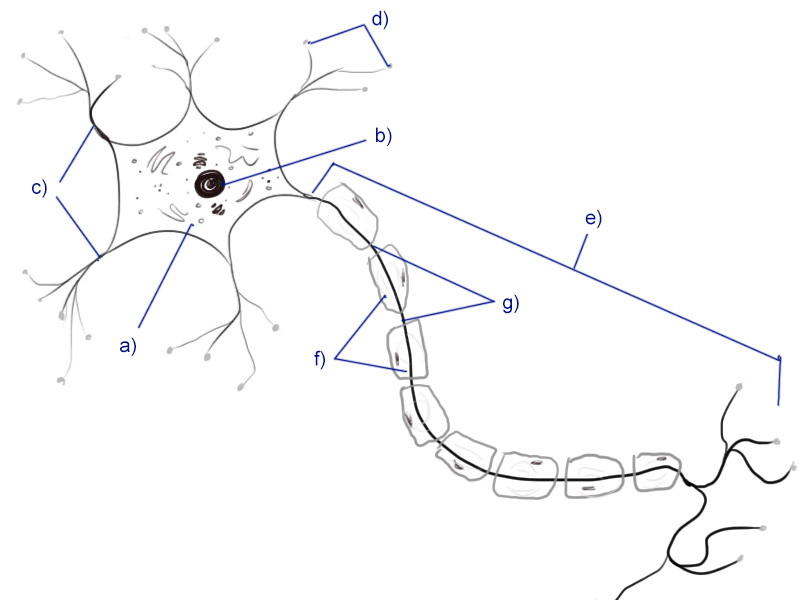
\includegraphics[width=0.7\textwidth]{img/neuron.jpg}}
		\caption{Grafika przedstawiająca schematyczną budowę neuronu na podstawie danych z ~\cite{neurology}.\\ 
		a)Soma/perykarion - ciało neuronu zawierające SER, RER, aparaty Golgiego, neurotubule i neurofilamenty, rybosomy, mitochondria, a także b) jądro komórkowe, c)dendryty, d)synapsy, e)neuryt/axon, f)osłonka mielonowa, g)przewężenia Ranviera  }
		\label{fig:neuron}
	\end{figure}
	Neuron jest jednostką morfologiczno-czynnościową układu nerwowego zbudowaną według schematu przedstawionego na  rys.~\ref{fig:neuron}. Dendryty odpowiedzialne są za przewodzenie impulsów elektrycznych pobranych przez synapsy w kierunku somy - ciała komórki nerwowej. Wyprowadzeniem impulsu zajmuje się akson - wypustka osiowa. Kierunek przebiegu jest zawsze stały  - mówi o tym prawo laryzacji dynamicznej. ~\cite{anatomy}\\ 
Przemieszczanie się impulsu elektrycznego zachodzi dzięki pompie sodowo-potasowej, która utrzymuje w komórce stałe napięcie powierzchniowe na błonie komórkowej. Potencjał spoczynkowy dla komórek nerwowych mieści się między -60, a -90mV, natomiast gdy dochodzi do pobudzenia komórki błona posiada potencjał czynnościowy, który mieści się między +20-50mV~\cite{neurology}. Właśnie dzięki postępującej różnicy potencjałów dochodzi do przewodzenia impulsu od dendrytu do aksonu i tym sposobem do kolejnego neuronu lub narządu wykonawczego.
\subsection{Podział układu nerwowego}
Układ nerwowy można podzielić najogólniej na układ somatyczny oraz autonomiczny. W skład pierwszego wchodzi ośrodkowy układ nerwowy oraz obwodowy układ nerwowy. Ośrodkowym układem nerwowym nazywa się mózgowie wraz z rdzeniem kręgowym, a obwodowym nerwy oraz zwoje. Schematyczny obraz układu nerwowego przedstawiono na rys.~\ref{fig:nervesystem} - kolorem czerwonym centralny układ nerwowy, niebieskim obwodowy układ nerwowy. Układ autonomiczny składa się z układu współczulnego i przywspółczulnego. \\
\begin{figure}[!h]

		\centering		
		 \scalebox{0.7}{
		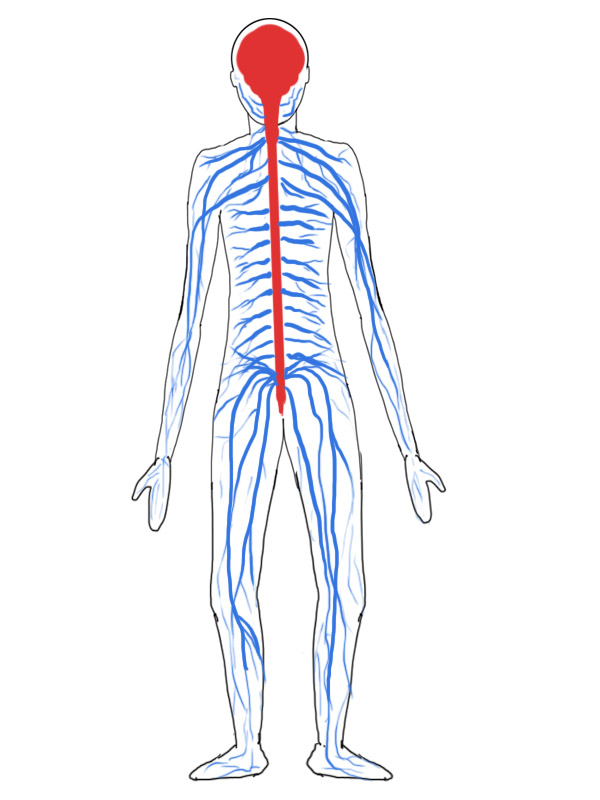
\includegraphics[width=0.7\textwidth]{img/nervesystem.jpg}}
		\caption{Grafika przedstawiająca schematyczną budowę układu nerwowego. }
		\label{fig:nervesystem}
	\end{figure}
	
Nerwy z kolei rozróżnia się ze względu na kierunek przewodnictwa na nerwy ruchowe można podzielić na ruchowe (tkzw. motoneurony) oraz czuciowe, lub też mieszane - ruchowo-czuciowe. Zgrupowanie komórek nerwowych poza ośrodkowym układem nerwowym nazywa się zwojem. 

	
	

\section{Zanikowe  stwardnienie boczne (ALS)}
\subsection{ Opis jednostki chorobowej}

Zanikowe stwardnienie boczne ( ang. amyotrophic lateral sclerosis ALS, łac. sclerosis lateralis
amyotrophica SLA) jest rzadką chorobą neurologiczną, dotyczącą  w 75\% przypadków zachorowań mężczyzn między 40 a 65 rokiem życia. ~\cite{neurology} Jednakże termin ALS jest używany do określania więcej niż jednego schorzenia związanego z degeneracją neuronów ruchowych.  Najczęściej stosowany jest, gdy mowa jest o klasycznej formie ALS (choroba Charcota), ale także w przypadku: Postępującego Porażenia Opuszkowego (Progressive bulbar palsy (PBP)), Postępującego Zaniku Mięśni (Progressive muscular atrophy (PMA)), Pierwotnego Stwardnienia Bocznego (Primary lateral sclerosis  (PLS)), Syndromu Ramienia Cepowatego (Flail arm syndrome (Vulpian-Bernhardt syndrome)), Syndromu Nogi Cepowatej (Flail leg syndrome  (Pseudopolyneuritic form)) oraz ALS  z powikłaniami wielonarządowymi  (np. ALSDementia) ~\cite{alsWij}. W celu ujednolicenia nazewnictwa Lord Russell Brain zaproponował termin Chorób Neuronu Ruchowego (Motor Neurone Disease (MND)). ~\cite{alsWij}\\
Istotą choroby jest zwyrodnienie komórek nerwowych odpowiedzialnych za przekazywanie sygnałów, wynikiem czego jest atrofia unerwianych przez nie mięśni. Degenerują neurony kory motorycznej (górny motoneuron), oraz neurony ruchowe rogów brzusznych rdzenia kręgowego, lub rdzenia przedłużonego (opuszki) (dolny motoneuron). Objawia się to początkowo ich osłabieniem, a ostatecznie zanikiem (przy czym same komórki mięśniowe nie obumierają, a jedynie zmniejszają swój rozmiar), co skutkuje ograniczeniem ruchów chorego, między innymi: gryzienia, chodzenia, mówienia i oddychania. ALS nie atakuje układu pokarmowego oraz krwionośnego. Swoją funkcjonalność stosunkowo długo zachowują neurony jądra Onufa unerwiające pęcherz moczowy i jądro nerwu okoruchowego odpowiedzialnego za ruchy gałek ocznych. Drogi czuciowe i sprawność intelektualna są zachowane. ~\cite{parkinsonALS} Powoduje to, że pacjent jest więźniem we własnym ciele - często nie mogącym się skomunikować z otoczeniem.  Co więcej ciągła świadomość pogarszającego się stanu chorego znacząco wpływa na jego samopoczucie i zdrowie psychiczne, prowadząc do depresji. \\
Nieznane są przyczyny zachorowań, jednak autorzy publikacji ~\cite{alsWij} oraz ~\cite{motoneuron} są zdania iż ALS jest wynikiem wzajemnego oddziaływania wielu czynników takich jak: czynniki genetyczne (między innymi dziedziczny defekt genu odpowiedzialnego za syntezę enzymu- desmutazy ponadtlenku Cu/Zn. [~\cite{neurology}-~\cite{alsWij}]), ekscytotoksyczność (patologiczny proces, w którym neurony są uszkadzane i zabijane przez aminokwasy o charakterze kwasowym m.in. glutaminian), stres oksydacyjny (gromadzenie reaktywnych form tlenu, na skutek zakłócenia równowagi pomiędzy ich wytwarzaniem, a biologiczną zdolnością do szybkiej detoksykacji, co prowadzi do obumierania komórek), dysfunkcje mitochondrialne (nieprawidłowości zarówno w ich budowie jak i funkcji), ograniczony transport aksonalny, anormalne gromadzenie neurofilamentów (to grupa białek włókienkowych stanowiących jeden z głównych komponentów cytoszkieletu komórek nerwowych), agregacja białek w cytoplazmie w postaci wtrętów, zaburzenia układu odpornościowego, reakcje autoimmunologiczne oraz niedobór neurotransmiterów.
ALS jest chorobą postępującą, co oznacza, że wraz z biegiem czasu następuje nasilenie objawów, w tym całkowita utrata kontroli nad ruchami dobrowolnymi. Na dzień dzisiejszy jest nieuleczalna i prowadzi do śmierci chorego w przeciągu 1-2 lat (25\% chorych). Jednak należy pamiętać, że SLA w swoim przebiegu jest chorobą bardzo indywidualną, więc tzw. okres przeżycia może wahać się w szerokich granicach. Ponad 25\% chorych przeżywa więcej niż 5 lat, w tym ok. 5\%  powyżej 10 lat .~\cite{poradnik}
\subsection{Próby terapii chorych.}

Do tej pory nie został znaleziony sposób skutecznego leczenia przyczynowego ALS. Jedynym lekiem o sprawdzonej skuteczności i dopuszczonym do stosowania w terapii  jest Rilutek (Riluzole, benzotiazol). Autorzy książki ~\cite{alsAdamek} poświęconej schorzeniu donoszą, że  „Badania  naukowe  dowodzą, że leczenie Riluzolem w dawce 100 mg dziennie (2x50 mg) przez 18 miesięcy nieznacznie  wydłuża  przeżycia  chorych  (średnio 3 – 4 miesiące)  niestety  nie  wpływając  na  poprawę  ich  stanu  klinicznego  i  jakości życia.”.  Terapia farmakologiczna chorych na ALS sprowadza się więc do leczenia objawowego.  

Innym ważnym aspektem terapii chorego jest odpowiednia rehabilitacja. Zwiększenie zakresu ruchów chorego oraz jak najdłuższe utrzymanie jego zdolności do samodzielnego wykonywania codziennych czynności jest głównym zadaniem specjalistycznej rehabilitacji ruchowej, która powinna być prowadzona od momentu diagnozy. Przykładowo wykonywane są: ćwiczenia w sali gimnastycznej, zajęcia ruchowe w basenie wzmacniające odpowiednie grupy mięśni, ćwiczenia czynne na sali chorych (chodzenie w balkonikach, stabilizatorach), czy też ćwiczenia bierne w łóżku chorego połączone z masażem leczniczym u pacjentów bez spastycznego napięcia.~\cite{alsAdamek} Korzystne efekty mogą wywoływać też takie zabiegi jak hydroterapia, kąpiele cieplne, elektroterapia, krioterapia. ~\cite{poradnik}\\
Z powodu utraty kontroli nad aparatem mowy komunikacja z chorym może stać się ograniczona, lub wręcz niemożliwa, dlatego lekarze, logopedzi i opiekunowie pacjenta mają za zadanie jak najdłuższe utrzymanie komunikacji.  Mowa tu nie tylko o komunikacji werbalnej, ale o nowych metodach wypracowywanych  indywidualnie przez chorego i opiekuna. 
Przy  narastających  zaburzeniach  dyzartrycznych  wykorzystuje  się metody  systemu  ACC  (ang.  Augmentive  and  Alternative  Communication  System)  czyli  wspomagającego  zastępczego  systemu  komunikacji,  zwiększającego możliwości komunikacyjne.~\cite{alsAdamek}

\section{Augmentative and Alternative Communication System}


Augmentative and alternative communication (AAC) jest dziedziną badań klinicznych oraz edukacyjnych. Głównym założeniem jest próba zgłębienia oraz kompensacji, gdy to konieczne, tymczasowych lub trwałych upośledzeń, czy też ograniczeń ze względu na możliwość posługiwania się oraz rozumienia komunikacji werbalnej oraz pisemnej.  Najczęstszymi przyczynami sięgania do tych metod komunikacji są: upośledzenia umysłowe, mózgowe porażenie dziecięce, autyzm oraz postępująca apraksja mowy ~\cite{augmentative} (jak w przypadku ALS). Zadaniem AAC nie jest jedynie wprowadzenie możliwości komunikacji osób chorych z otoczeniem, ale także umożliwienie im czynnego udziału w życiu społecznym oraz towarzyskim, wykonywania czynnego zawodu, czy też poświęcaniu się hobby jak pisanie prozy, bądź poezji, co w sposób znaczący odbija się na ich samopoczuciu oraz jakości życia. Dąży się zatem do zapewnienia tego podstawowego prawa każdemu pacjentowi. 


	ACC polega na wymianie wiadomości, które muszą zostać sformułowane, przechowane oraz odzyskane w dowolnym momencie. Wiadomością może być pojedyncze słowo, kod lub też struktury bardziej złożone mające na celu podtrzymanie komunikacji interpersonalnej, pisanej – także tej na mediach społecznościowych, które w dzisiejszych czasach stanowią ważny filar interakcji międzyludzkich.
\\ Istnieje kilka metod formowania pełnych zdań : jedną z nich jest wpisywanie wiadomości znak po znaku, inną jest korzystanie z gotowych bibliotek wyrazów. Możliwe jest także wykorzystanie już gotowych wzorów pełnych, lub części zdań – co zdecydowanie przyspiesza komunikację, jednak metoda ta jest ograniczona przez pamięć biblioteki przechowującej takie wzorce. Biblioteka taka tworzona i kompletowana jest zgodnie z indywidualnymi potrzebami chorego i zależy od jego płci, wieku, zawodu, stylu życia itp. Dla dzieci przygotowywane są specjalne tablice obrazkowe, które pozwalają im na jasny przekaz. \\
Tablice można podzielić ze względu na ich ułożenie obiektów na statyczne oraz dynamiczne. W tablicach statycznych każdy obiekt ma swoje ustalone położenie, które nie zmienia. Do komunikacji niezbędna jest więc duża ilość statycznych tablic – przykładem są tablice fizyczne – papierowe, gdzie nie można zmieniać położenia wydrukowanych na kartce elementów. Dynamiczne wyświetlacze odnoszą do się wyświetlaczy komputowych, w których dzięki odpowiedniemu oprogramowaniu, można dynamicznie poruszać się między widokami.  
W celu ułatwienia korzystania z bibliotek zebranych w tablice istnieje kilka metod przedstawionych w ~\cite{augmentative}.
\begin{enumerate}
\item Semantic-Syntactic Grid Displays (Semantyczno-syntaktyczna siatka/tablica) – tablica cechująca się podziałem wyświetlanych na niej słów na kategorie, zazwyczaj ze względu na części mowy. Możliwe jest także przedstawienie słów w logicznej kolejności występowania w zdaniu. Przykładowym algorytmem sortowania jest klucz Fitzgeralda – słowa układa się od lewej do prawej, układając je w klasy odpowiadające na pytania: „Kto?”, „Co robi?”, „Co?”, „Gdzie?”, „Jaki?”, „Kiedy?” itd.  Słowa, bądź litery najczęściej wybierane układane są w pierwszym bądź ostatnim wierszu tablicy. Elementem stanowczo usprawniającym korzystanie było kolorowanie elementów zgodnie z ich przynależnością do  klasy. 
\item Taxonomic Grid Displays (Siatka/tablica taksonomiczna) – dzieli słownictwo na klasy: osoby, miejsca, uczucia, jedzenie, napoje, słowa opisujące czynności. Nie jest to rekomendowany typ tablic dla dzieci w wieku poniżej 6 roku życia. 
\item Activity Grid Displays ( Tablica/siatka czynności) – najpopularniejszy typ tablic. Kategoryzacja słownictwa następuje ze względu na rodzaj czynności, wydarzenia, czy rutyny, której ono dotyczy np. „zakupy” lub „płacenie przy kasie”, czy też „rozmowa ze sprzedawcą”. Każda kategoria jest podzielona jak wyżej na mniejsze podklasy ze względu na to, co dane słowo określa. 
\item Pragmatic Organization Dynamic Display (Dynamiczny wyświetlacz  struktur pragmatycznych) – metoda kładącą duży nacisk na efektywność komunikacji, w tym celu stosując kombinację kilku różnych strategii organizacji słownictwa. 
\item Visual Scene Displays (Wyświetlacz obrazkowy) – słownictwo posortowane jest według przynależności do czynności lub rutyny, które zobrazowane są w postaci  symbolu kojarzącego się z nimi. Rozmieszczenie tych grafik nie jest siatkowe, a metodyczne. Takie rozwiązanie wykazało się wyjątkowo skuteczne w pracy z małymi dziećmi, które w bardzo krótki czasie opanowały taką formę komunikacji.  Zauważono także większą chęć interakcji w przypadku korzystania z tej formy niż w przypadku korzystania z tablic. 
\item Hybrid Display ( Wyświetlacz hybrydowy) – połączenie metody wyświetlacza obrazkowego oraz tablic. Przedstawia się zdjęcie,  na którym zaznaczone są elementy i wyświetlone związane z nimi słowa np. na obrazku widać osobę, więc wyświetlane będą np. części ciała, czynność jaka ta osoba wykonuje, emocje itp. 
 \ldots
\end{enumerate}
Ze szczególnym przypadkiem, który wymaga osobnego traktowania, mamy do czynienia w przypadku osób dorosłych z nabytą niepełnosprawnością- jak ma to miejsce w wypadku chorych na ALS. 93\% osób chorujących jest uzależniona od metod AAC .  Dorośli potrzebują więcej czasu, żeby przestawić się i przyzwyczaić się do niewerbalnej komunikacji, dlatego też zalecana im jest nauka korzystania np. z tablic od razu po diagnozie, nawet jeśli chory jest jeszcze w pełni sprawny. Zmiana stanu zdrowia w wypadku tej jednostki może nastąpić w bardzo krótkim czasie.   

\section{Technologiczne rozwiązania dla chorych na ALS}

Jak wyżej wspomniano, do rozwiązań dla chorych na ALS należą statyczne oraz dynamiczne tablice, jednak aby się nimi posługiwać należy albo opracować metodę AAC  np. dwa mrugnięcia oznaczają tak, a jedno nie, lub wykorzystać sygnały płynące z organizmu ludzkiego jako wskaźniki. Do mierzonych wartości należą m.in. impulsy elektryczne pochodzące z mózgu (mierzone za pomocą EEG), mięśni (mierzone za pomocą EMG) lub detekcja mikroruchów kończyn.~\cite{eyemouse} Ze względu na to, że technologie wykorzystujące  EEG wymagają bardzo stabilnych warunków elektromagnetycznych i są niezwykle czułe na szum, nie są optymalnymi rozwiązaniami dla chorych na ALS. Metodą bardzo dobrze się sprawdzającą, ze względu na długie zachowanie funkcjonalności gałek ocznych, jest EGT, czy też eye-tracking, czyli śledzenie wzroku. Jest to metoda bardziej niezawodna niż wyżej wymienione. 
\subsection{Eye-tracking} 

Eye-tracking, znany również jako okulorografia,  ma za zadanie np. określenie ruchów gałek ocznych, a przez to  punktu fiksacji wzroku,  najczęściej w czasie rzeczywistym. Do metod pozwalających na śledzenie wzroku oraz ruchów oczu należy m.in. elektrookulografia, śledzenie ruchu gałek ocznych, powiek, metody działające w oparciu o szkła kontaktowe, metody wykorzystujące refleksy na rogówce lub źrenicy~\cite{eyemouse}. Do poprawnego działania wymienionych metody najczęściej niezbędny jest również pomiar ruchów głowy.
\\ Technologia ta wykorzystywana jest często podczas badań marketingowych do określenia skuteczności reklamy – ustalenia, co przyciąga największą uwagę odbiorcy, bądź w celu orzeczenia poziomu użyteczności zaprojektowanego interfejsu.
Coraz częściej implementuje się dane techniki  np. w grach,  w medycynie m. in. w celu umożliwienia korzystania z urządzeń ekranowych osobom z upośledzeniami fizycznymi, które ich przed tym powstrzymują oraz wszędzie tam, gdzie użytkownik nie może mięć zajętych rąk. We współpracy z urządzeniami elektronicznymi takimi jak  komputer lub urządzenia mobilne osoba upośledzona, bądź chora może w sposób znaczący poprawić swoją jakoś życia. W celu sprawnej współpracy niezbędne jest dokładne określenie punktu fiksacji wzroku (punktu, na którym użytkownik skupia swój wzrok przez co najmniej 0,15s)~\cite{kunkaUwaga}.
\subsubsection{Podział urządzeń do eye-trackingu}

Z przykładem bardzo dobrego podziału urządzeń można zapoznać się na materiałach wykładowych pana dr inż. Bartoszka Kunki ~\cite{kunkaFiksacja}. Według niego pierwszym kryterium podziały powinna być mobilność urządzenia pomiarowego na: mobilne i niemobline, gdzie do pierwszych zaliczyć można wszystkie urządzenia nagłowne np. smartglasses, a do drugich urządzenia stacjonarne – związane na stałe np. z monitorem lub zamontowane na stojakach – mam wtedy do czynienia najczęściej z urządzeniami bezdotykowymi. Urządzenia mobilne bazują na technice wykorzystujące podczerwień, natomiast stacjonarne mogą, prócz wyżej wspomnianej, monitorować badane parametry również niezależnie od światła  IR – wykorzystując światło dzienne. 

\paragraph{Działanie urządzeń opartych na oświetleniu w podczerwieni. [~\cite{kunkaFiksacja}, ~\cite{erica}]}\leavevmode\\
W celu obserwacji ruchów gałki ocznej i określenia punktu fiksacji należy oko naświetlać światłem punktowym w podczerwieni albo w linii zgodnej z osią kamery, bądź poza nią i w zależności od wybranej metody zauważa się inne zjawiska optyczne. Podczerwień powoduje znaczy wzrost kontrastu między tęczówką, a źrenicą oka, co pozawala na dokładniejsze określenie pozycji źrenicy, co wyznaczane jest na podstawie odbicia obserwowanego na nagraniu tworzonym przez kamerę, która przez cały czas działania aparatury  skierowana jest na jedno z oczu osoby badanej~\cite{erica}.
Wśród obserwowanych odbić najbardziej istotnym względem badanego aspektu jest tzw. glint (błysk na rogówce, powstający, gdy dioda jest poza osią kamery). Glint, znany również jako  pierwszy obraz Purkinjego [~\cite{kunkaFiksacja},~\cite{erica}], nie zmienia swego położenia wraz z ruchami gałki ocznej – dlatego uważany jest jako punkt referencyjny, tak dług, jak głowa badanej osoby pozostaje nieruchoma względem kamery.  Diody umieszczone na osi kamery wywołują zjawisko jasnej źrenicy ~\cite{kunkaFiksacja} – część podczerwonego światła przedostaje się do źrenicy i zostaje od niej odbita, wywołując efekt  przypominający np. kocie oko oświetlone w ciemności.  Porównując więc pozycję glinta (lub glintów) oraz ruchomej jasnej źrenicy jesteśmy w stanie na podstawie ich względnego położenia określić punkt fiksacji oka. Określenie kierunku skierowania wzroku na podstawie względnego położenia glintu oraz źrenicy na grafice  ~\ref{fig:glint}. Schemat algorytmu wyznaczania punktu fiksacji przedstawiono na rysunku ~\ref{fig:glintUML} opartym na materiałach wykładowych ~\cite{kunkaFiksacja}.

\begin{figure}[!h]
		\centering
		\scalebox{.7}{
		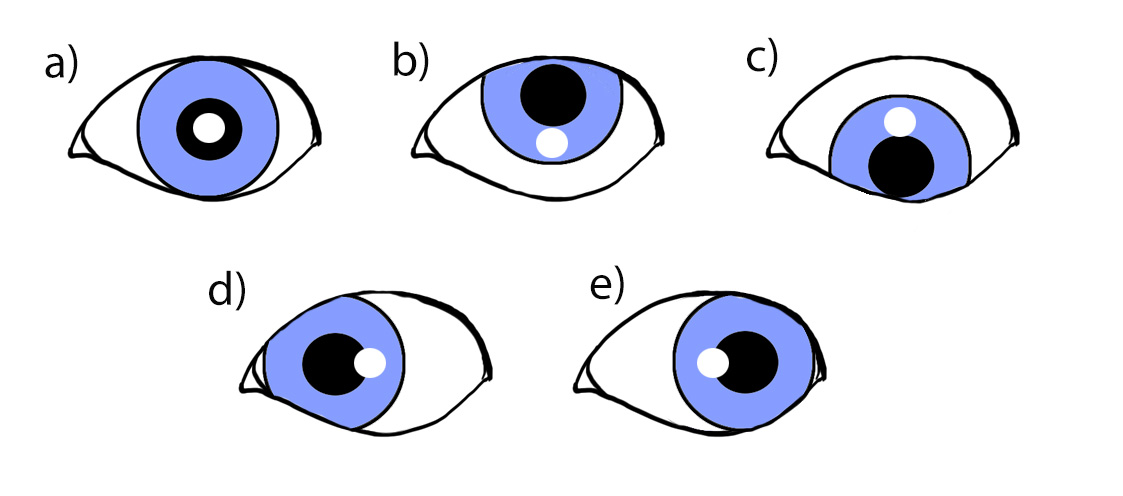
\includegraphics[width=0.7\textwidth]{img/glint.jpg}}
		\caption{Położenie glinta względem środka źrenicy w zależności od ruchu gałki ocznej. \\
a) patrzenie prosto w źródło światła b) patrzenie powyżej źródła światła c) patrzenie poniżej źródła światła d)patrzenie w lewo od źródła światła e)patrzenie w prawo od źródła światła 
}
		\label{fig:glint}
	\end{figure}
	
\begin{figure}[!h]

		\centering		
		 \scalebox{.65}{
		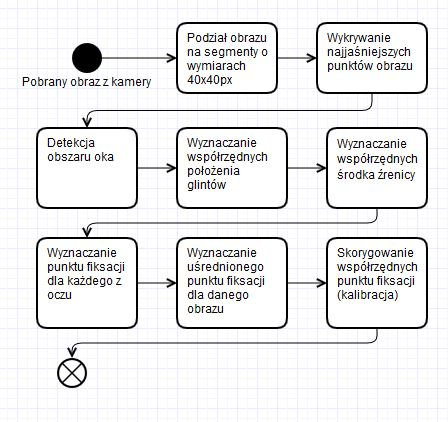
\includegraphics[width=0.7\textwidth]{img/UMLglint.jpg}}
		\caption{Poglądowy schemat algorytmu wyznaczania punktu fiksacji przy wykorzystaniu światła IR. }
		\label{fig:glintUML}
	\end{figure}
	
Odległości wyliczane są  na postawie obrazów przechwyconych  przez kamerę i przetworzonych komputerowo.  
Tą samą technologię można również zmodyfikować, by wyznaczać punkt fiksacji  z położenia 4 glintów ( wywołanych 4 diodami rozmieszczonymi w narożnikach ekranu) lub przy zastosowaniu skomplikowanych  przekształceń matematycznych,  poprawiających dokładność  wyznaczenia punktu fiksacji. ~\cite{kunkaFiksacja}
Inną metodą – wykorzystującą  na przemian dwa rodzaje diod ( na lub poza osią kamery) jest metoda różnicowa ~\cite{kunkaFiksacja}. Wykorzystuje się kolejne klatki nagrania, przy czym jedna klatka zawiera efekt jasnej źrenicy, a druga zawiera efekt ciemnej źrenicy i glinty. Punkt fiksacji po raz kolejny jest wynikiem różnicy odległości obu zjawisk i obliczany jest na podstawie wynikowego obrazu różnicowego.\\
Przykładami technologii, które do tej pory wykorzystały powyższy algorytm to np. Erica[1989].
\paragraph{Działanie urządzeń  opartych na świetle dziennym. }\leavevmode\\
W przypadku  metod  wykorzystujących światło dzienne i kamerę rejestrujące ruchy gałek ocznych mamy do czynienia z bardzo złożonymi algorytmami komputerowymi, które pozwalają na przetwarzania obrazu powodującego określenie punktu fiksacji wzroku. Wraz z zaletą, jaką jest brak zapotrzebowanie na dodatkowy sprzęt (algorytmy mogą współpracować z wbudowanymi kamerkami komputerowymi), technologie te niestety często charakteryzują się gorszą dokładnością.

Przykładem technologii korzystającej ze światła dziennego jest Eye Mouse – projekt powstały na terenie Politechniki Gdańskiej ~\cite{eyemouse}, którego głównym założeniem jest wykorzystanie wzroku jako zastępstwo myszy komputerowej oraz klawiatury.W tym celu wykorzystuje się dwie kamery – jednej śledzącej wzrok, a drugiej położenie głowy osoby badanej względem ekranu – tak, że na otrzymywany wynik nanoszona jest korekta.  W rogach ekranu umieszczone są 4 diody światła podczerwonego jako znaczniki. W procesie przetwarzania obrazów usuwany jest szum oraz wyznaczana jest źrenica oraz jej środek. Kolejnym krokiem jest oznaczenie wzajemnej zależności pozycji ekranu względem głowy osoby badanej – w tym celu wykorzystuje się znaczniki LED. Proces ten niezbędny jest w celu kalibracji.
\section{Podsumowanie}
Zapoznawszy się z problematyką choroby zanikowego stwardnienia bocznego oraz z możliwościami technologicznymi oferowanymi pacjentom można przejść do stworzenia aplikacji komputerowej, która ma za cel ułatwienie komunikacji chorych z komputerem. Wykorzysta się do tego metodę eye-trackingu korzystającej ze światła dziennego - zwiększając w ten sposób dostępność oraz uniwersalność aplikacji. 

\end{document}

